\documentclass{standalone}
\usepackage{tikz}
\begin{document}
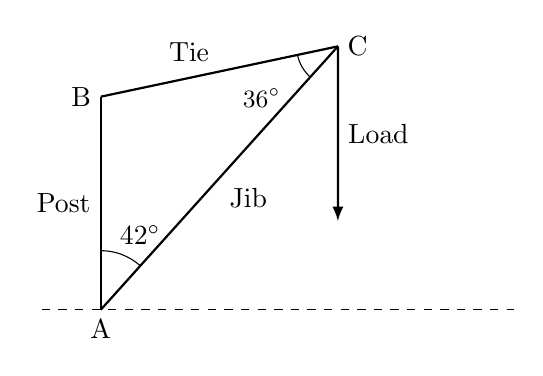
\begin{tikzpicture}[scale=1.5]
  % Coordinate definitions
  \coordinate (A) at (0,0); % Post base
  \coordinate (B) at (0,1.8033); % Tie attachment on post
  \coordinate (C) at ({3*cos(48)},{3*sin(48)}); % Crane head (jib length 3, 48° to horizontal)

  % Draw post
  \draw[thick] (A) -- (B) node[midway, left] {Post};

  % Draw jib
  \draw[thick] (A) -- (C) node[midway, below right] {Jib};

  % Draw tie
  \draw[thick] (B) -- (C) node[midway, above left] {Tie};

  % Draw load
  \draw[thick, -latex] (C) -- ({3*cos(48)},0.75) node[midway, right] {Load};

  % Label points
  \node[below] at (A) {A};
  \node[left] at (B) {B};
  \node[right] at (C) {C};

  % Draw angles
  % Jib to vertical (42°) at A
  \draw (A) ++(0,0.5) arc (90:48:0.5) node[midway, above right, xshift=-1.5mm] {$42^\circ$};

  % Tie to jib (36°) at C, inside triangle in quadrant 3
  % CA: 228°, CB: 192°
  \draw (C) ++(228:0.35) arc (228:192:0.35) node[midway, below left, xshift=-1.5mm, yshift=-1.5mm, font=\small] {$36^\circ$};

  % Ground
  \draw[dashed] (-0.5,0) -- (3.5,0);
\end{tikzpicture}
\end{document}